\section{Технический проект}
\subsection{Общая характеристика организации решения задачи}

Задача заключается в разработке и программной реализации веб-приложения для управления проектами, основанного на использовании Kanban-доски и принципов Agile-методологий. Приложение предназначено для командной работы и поможет руководителям проектов, а также членам команд эффективно планировать спринты и текущую деятельность, визуализировать рабочие процессы, отслеживать выполнение задач и улучшать взаимодействие, что способствует повышению общей продуктивности и успешности проектов.

Приложение будет представлять собой многопользовательский веб-сервис, доступный через сеть Интернет. Основными элементами интерфейса будут являться интерактивная Kanban-доска для визуального управления задачами, страницы для настройки проектов и досок, а также инструменты для поддержки Agile-практик, такие как управление бэклогом и отслеживание прогресса по итерациям.

\subsection{Обоснование выбора технологии проектирования}

Для создания приложения выбраны технологии, которые обеспечивают высокую производительность и удобство для пользователей.

\subsubsection{Язык программирования JavaScript}
JavaScript — это высокоуровневый, мультипарадигменный язык программирования, являющийся ключевой технологией для создания интерактивных веб-сайтов и приложений. Он выполняется непосредственно в браузере пользователя, обеспечивая динамическое обновление контента и взаимодействие без перезагрузки страницы, а также может использоваться на серверной стороне благодаря среде Node.js \cite{javascript1}.

\subsubsection{Среда выполнения Node.js}
Node.js — это кроссплатформенная среда выполнения JavaScript, построенная на движке V8 от Google Chrome. Она позволяет исполнять JavaScript-код на стороне сервера, что открывает возможности для создания быстрых и масштабируемых сетевых приложений \cite{nodejs1}.

\subsubsection{Библиотека React}
React — это популярная JavaScript-библиотека для создания пользовательских интерфейсов, разработанная и поддерживаемая Facebook (ныне Meta). В основе React лежит концепция компонентного подхода, позволяющая разбивать сложный интерфейс на независимые, переиспользуемые части — компоненты, каждый из которых управляет собственным состоянием \cite{react1}.

\subsubsection{PostgreSQL}

PostgreSQL — это объектно-реляционная система управления базами данных, известная своей надежностью, гибкостью и расширяемостью. Она поддерживает широкий спектр функциональности, включая сложные запросы, транзакции, уровни изоляции и возможность создания пользовательских типов данных \cite{postgres1}.

\subsection{Диаграмма компонентов}

 На рисунке \ref{components_diagram.eps:image} изображена диаграмма компонентов системы.
 
 \begin{figure}[ht]
 	\center{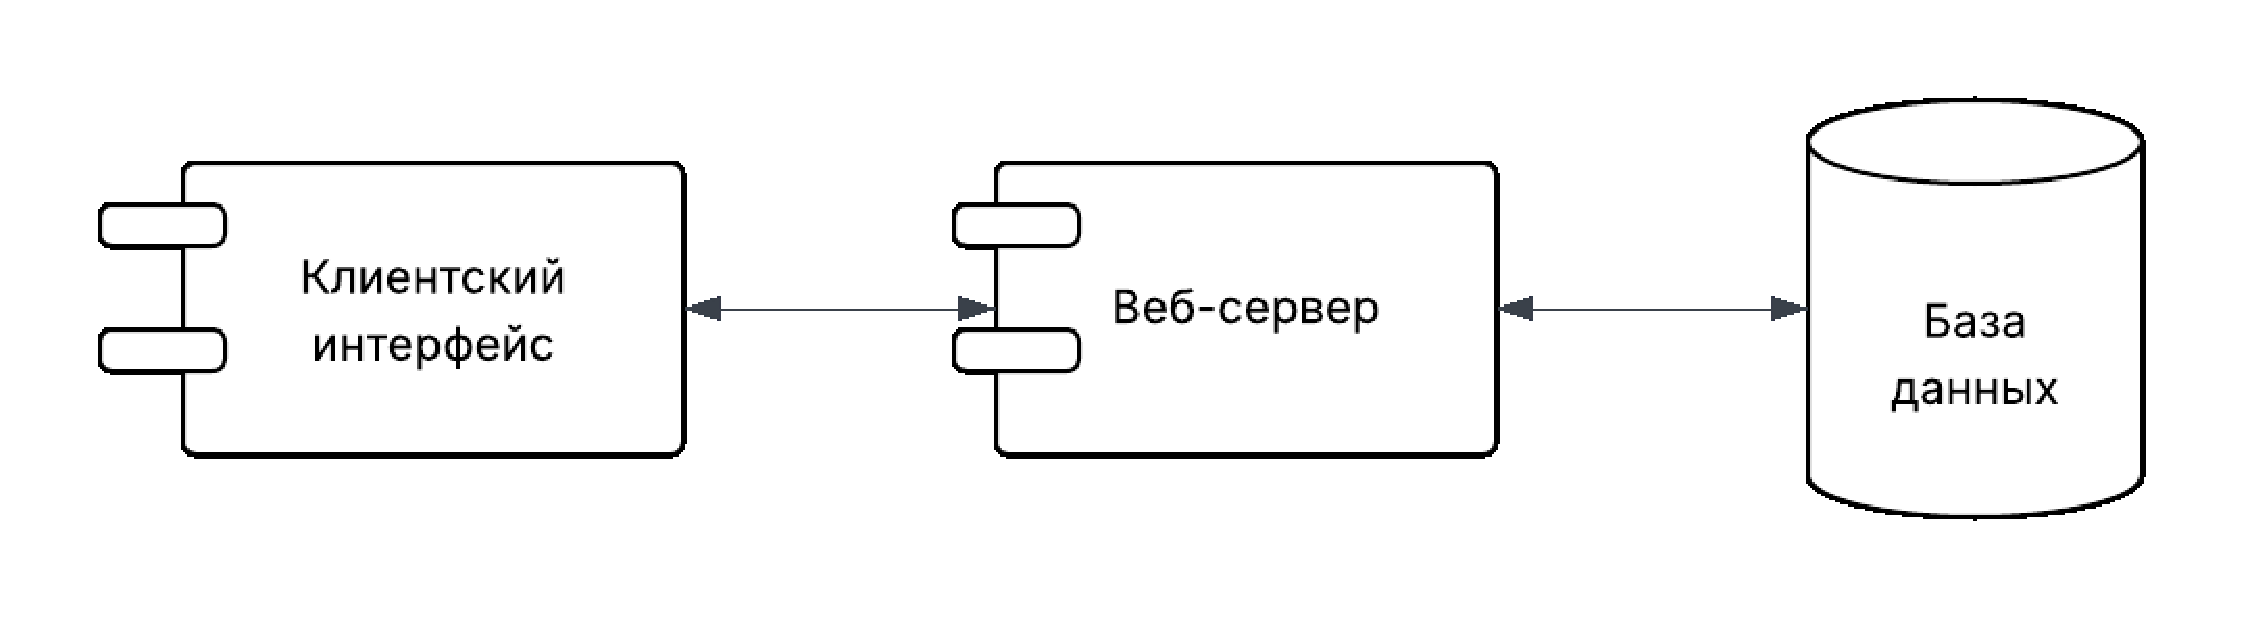
\includegraphics[width=1\linewidth]{components_diagram}}
 	\caption{Диаграмма компонентов}
 	\label{components_diagram.eps:image}
 \end{figure}
 
 На представленной диаграмме показана архитектура веб-приложения для управления проектами, основанного на Kanban-доске и Agile-методиках. Схема включает три основных компонента: «Клиентский интерфейс», «Веб-сервер» и «База данных». Эти компоненты соединены стрелками, которые указывают направление потоков данных и взаимодействия между ними. Каждая часть системы выполняет свои специфические функции, обеспечивая совместную и эффективную работу всего приложения.
 
 «Клиентский интерфейс» — это веб-приложение, которое запускается в браузере пользователя и служит основной точкой взаимодействия с системой. Через него пользователи могут регистрироваться и аутентифицироваться, создавать новые проекты, настраивать Kanban-доски, добавлять, редактировать и перемещать задачи между колонками. На страницах интерфейса в реальном времени отображается актуальное состояние проектов, Kanban-доски, списки задач, бэклоги и другая информация, необходимая для организации работы по Agile-принципам.
 
 «Веб-сервер» функционирует как центральный узел архитектуры, обрабатывающий всю бизнес-логику системы. Он получает HTTP-запросы от «Клиентского интерфейса», выполняет соответствующие операции, взаимодействует с «Базой данных» для сохранения или извлечения необходимой информации, и отправляет ответы «Клиентскому интерфейсу» для обновления отображаемых данных или подтверждения выполненных действий.
 
 «База данных» отвечает за надежное и долговременное хранение всей информации, используемой в системе управления проектами. В ней содержатся структурированные данные о зарегистрированных пользователях, созданных проектах, деталях задач, конфигурациях Kanban-досок и другие сведения, необходимые для функционирования Agile-процессов. «Веб-сервер» постоянно обращается к «Базе данных» для выполнения операций чтения и записи данных при каждом значимом взаимодействии пользователя с системой.

\subsection{Структура базы данных}

Сущности и отношения между ними отображены на ER-диаграмме.

 \begin{figure}[ht]
	\center{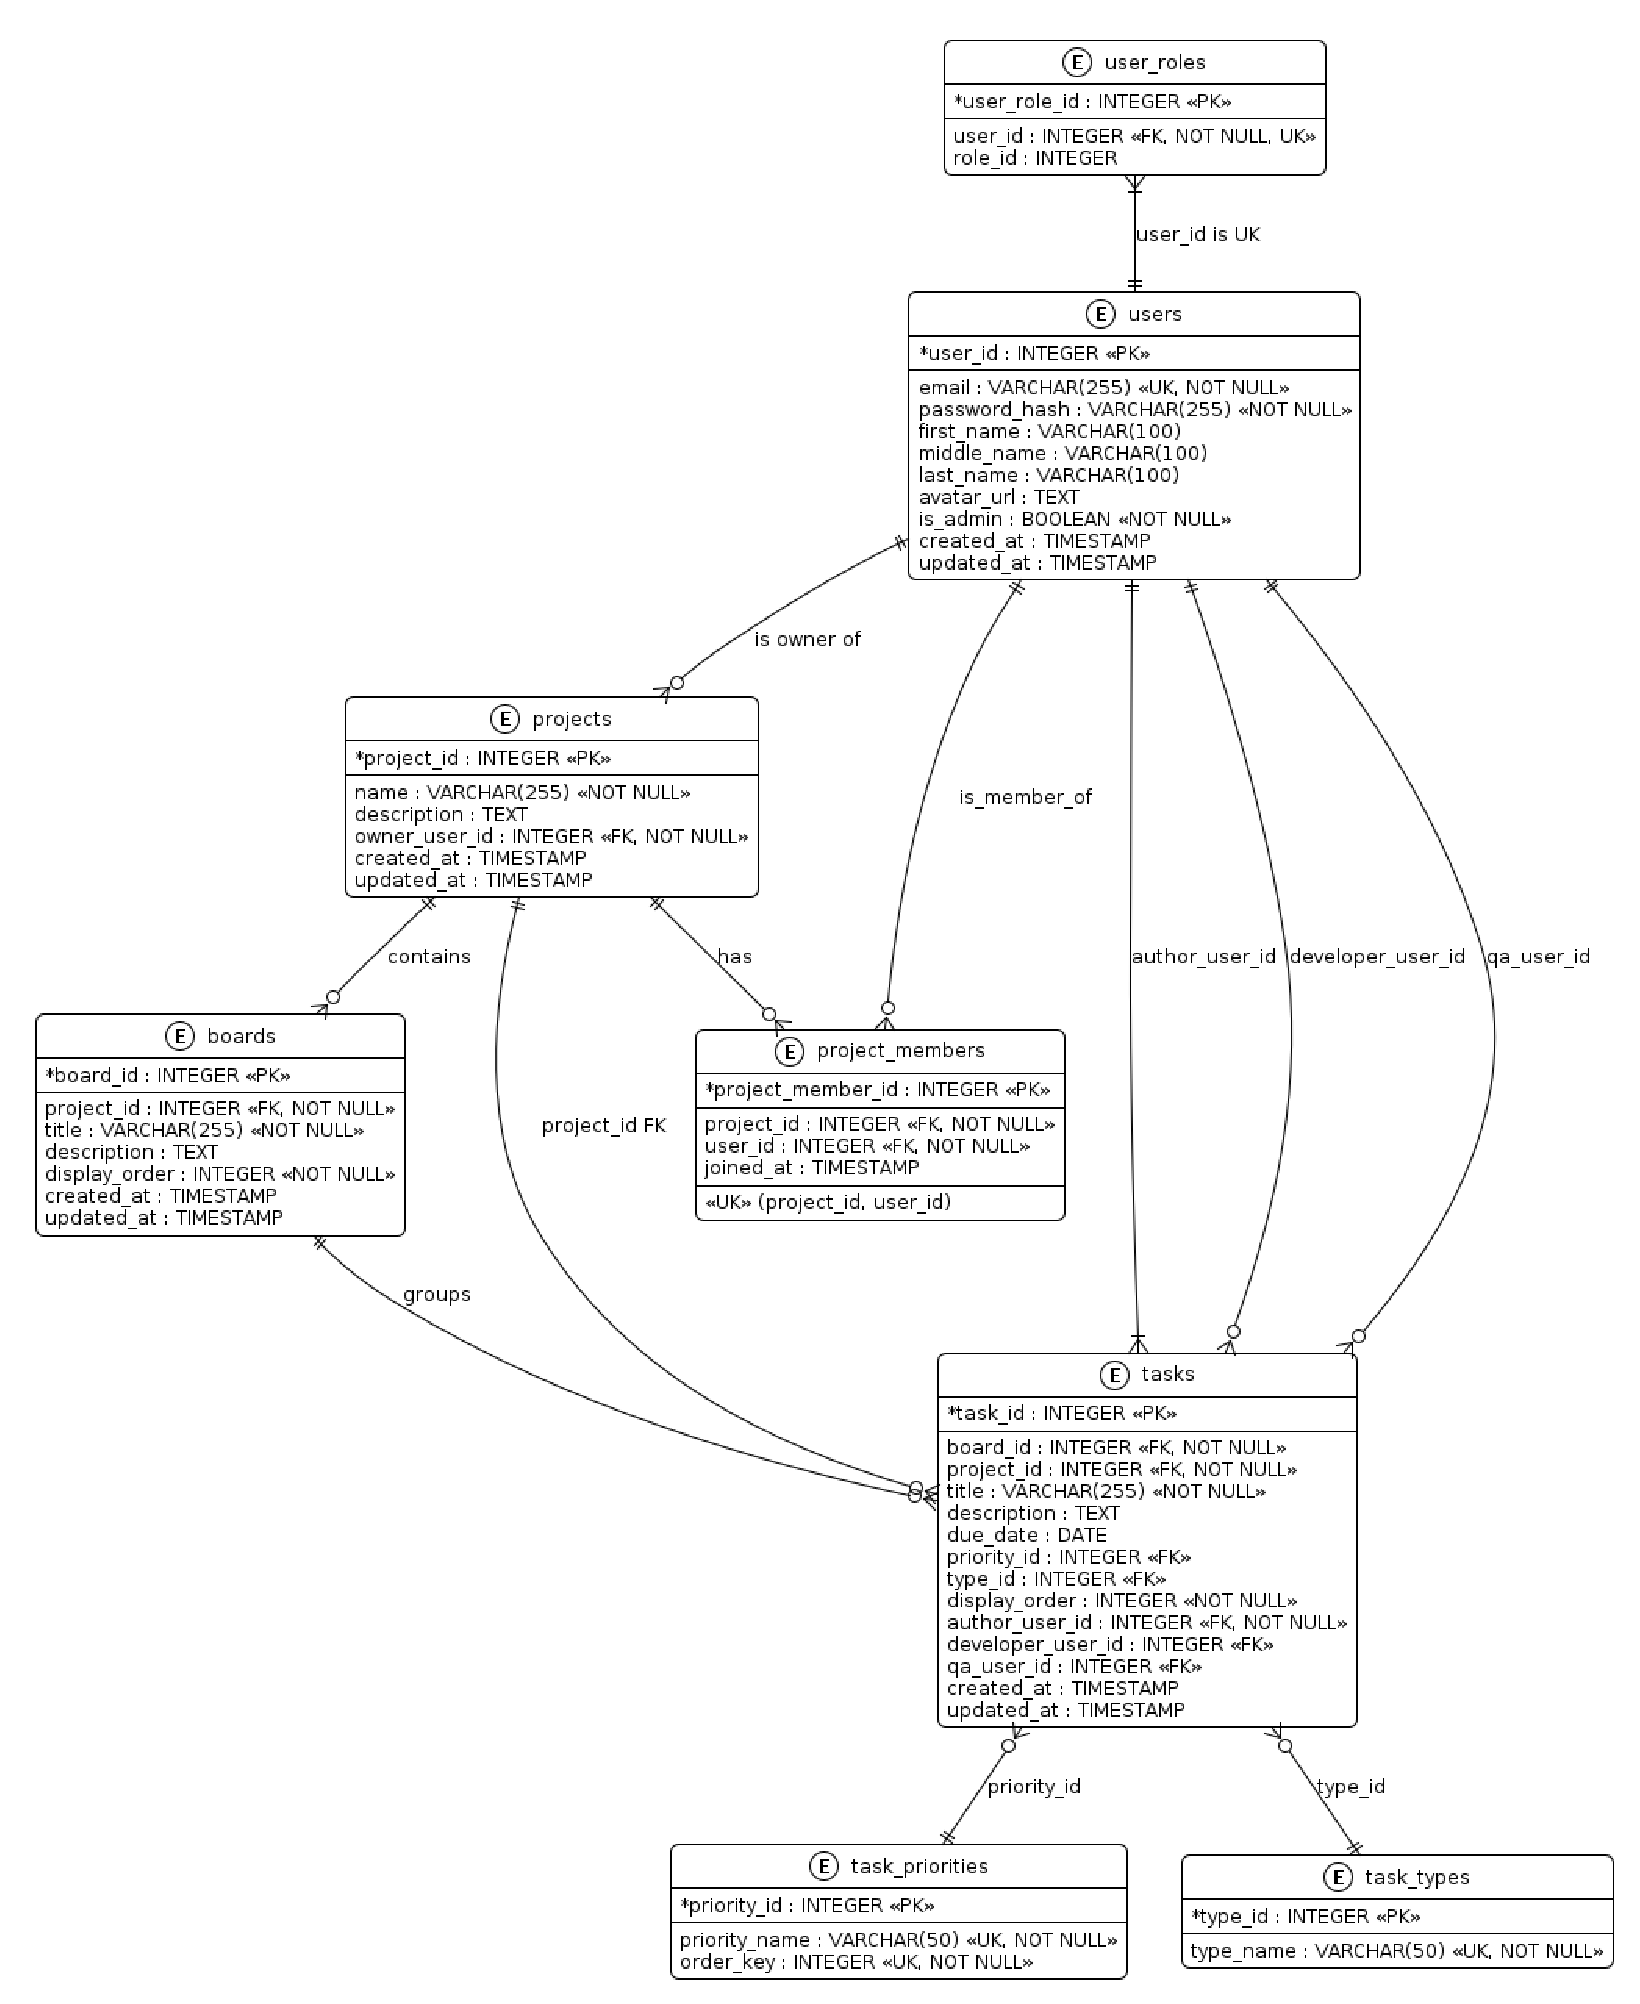
\includegraphics[width=1\linewidth]{er_diagram}}
	\caption{ER-диаграмма}
	\label{er_diagram:image}
\end{figure}

\begin{xltabular}{\textwidth}{|p{2.5cm}|p{4cm}|p{1.7cm}|X|}
	\caption{Атрибуты сущности «Users»\label{users:table}}\\ \hline
	\centrow Поле & \centrow Тип & \centrow Обяза\-тельное & \centrow Описание \\ \hline
	\thead{1} & \thead{2} & \centrow 3 & \centrow 4 \\ \hline
	\endfirsthead
	\caption*{Продолжение таблицы \ref{users:table}} \\ \hline
	\thead{1} & \thead{2} & \centrow 3 & \centrow 4 \\ \hline
	\finishhead
	user\_id & SERIAL, PK & \centrow да & Первичный ключ, уникальный идентификатор пользователя. \\ \hline
	email & VARCHAR(255), UNIQUE, NOT NULL & \centrow да & Адрес электронной почты пользователя, уникальный. \\ \hline
	password\_ hash & VARCHAR(255), NOT NULL & \centrow да & Хеш пароля пользователя. \\ \hline
	first\_name & VARCHAR(100) & \centrow нет & Имя пользователя. \\ \hline
	middle\_ name & VARCHAR(100) & \centrow нет & Отчество пользователя. \\ \hline
	last\_name & VARCHAR(100) & \centrow нет & Фамилия пользователя. \\ \hline
	avatar\_url & TEXT & \centrow нет & URL-адрес аватара пользователя. \\ \hline
	is\_admin & BOOLEAN, DEFAULT FALSE, NOT NULL & \centrow да & Флаг, указывающий, является ли пользователь администратором. \\ \hline
	created\_at & TIMESTAMP WITH TIME ZONE, DEFAULT CURRENT\_ TIMESTAMP & \centrow да & Дата и время создания записи. \\ \hline
	updated\_at & TIMESTAMP WITH TIME ZONE, DEFAULT CURRENT\_ TIMESTAMP & \centrow да & Дата и время последнего обновления записи. \\ \hline
\end{xltabular}

\begin{xltabular}{\textwidth}{|p{2.5cm}|p{4cm}|p{1.7cm}|X|}
	\caption{Атрибуты сущности «Projects»\label{projects:table}}\\ \hline
	\centrow Поле & \centrow Тип & \centrow Обяза\-тельное & \centrow Описание \\ \hline
	\thead{1} & \thead{2} & \centrow 3 & \centrow 4 \\ \hline
	\endfirsthead
	\caption*{Продолжение таблицы \ref{projects:table}} \\ \hline
	\thead{1} & \thead{2} & \centrow 3 & \centrow 4 \\ \hline
	\finishhead
	project\_id & SERIAL, PK & \centrow да & Первичный ключ, уникальный идентификатор проекта. \\ \hline
	name & VARCHAR(255), NOT NULL & \centrow да & Название проекта. \\ \hline
	description & TEXT & \centrow нет & Описание проекта. \\ \hline
	owner\_ user\_id & INTEGER, FK, NOT NULL & \centrow да & Внешний ключ, ссылается на users(user\_id). Идентификатор пользователя-владельца проекта. \\ \hline
	created\_at & TIMESTAMP WITH TIME ZONE, DEFAULT CURRENT\_ TIMESTAMP & \centrow да & Дата и время создания записи. \\ \hline
	updated\_at & TIMESTAMP WITH TIME ZONE, DEFAULT CURRENT\_ TIMESTAMP & \centrow да & Дата и время последнего обновления записи. \\ \hline
\end{xltabular}

\begin{xltabular}{\textwidth}{|p{2.5cm}|p{4cm}|p{1.7cm}|X|}
	\caption{Атрибуты сущности «Project Members»\label{projectmembers:table}}\\ \hline
	\centrow Поле & \centrow Тип & \centrow Обяза\-тельное & \centrow Описание \\ \hline
	\thead{1} & \thead{2} & \centrow 3 & \centrow 4 \\ \hline
	\endfirsthead
	\caption*{Продолжение таблицы \ref{projectmembers:table}} \\ \hline
	\thead{1} & \thead{2} & \centrow 3 & \centrow 4 \\ \hline
	\finishhead
	project\_ member\_id & SERIAL, PK & \centrow да & Первичный ключ, уникальный идентификатор записи об участии. \\ \hline
	project\_id & INTEGER, FK, NOT NULL & \centrow да & Внешний ключ, ссылается на projects(project\_id). Идентификатор проекта. \\ \hline
	user\_id & INTEGER, FK, NOT NULL & \centrow да & Внешний ключ, ссылается на users(user\_id). Идентификатор пользователя-участника. \\ \hline
	joined\_at & TIMESTAMP WITH TIME ZONE, DEFAULT CURRENT\_ TIMESTAMP & \centrow да & Дата и время присоединения пользователя к проекту. \\ 
	\hline
\end{xltabular}

\begin{xltabular}{\textwidth}{|p{2.5cm}|p{4cm}|p{1.7cm}|X|}
	\caption{Атрибуты сущности «Boards»\label{boards:table}}\\ \hline
	\centrow Поле & \centrow Тип & \centrow Обяза\-тельное & \centrow Описание \\ \hline
	\thead{1} & \thead{2} & \centrow 3 & \centrow 4 \\ \hline
	\endfirsthead
	\caption*{Продолжение таблицы \ref{boards:table}} \\ \hline
	\thead{1} & \thead{2} & \centrow 3 & \centrow 4 \\ \hline
	\finishhead
	board\_id & SERIAL, PK & \centrow да & Первичный ключ, уникальный идентификатор доски. \\ \hline
	project\_id & INTEGER, FK, NOT NULL & \centrow да & Внешний ключ, ссылается на projects(project\_id). Идентификатор проекта, к которому принадлежит доска. \\ \hline
	title & VARCHAR(255), NOT NULL & \centrow да & Название доски. \\ \hline
	description & TEXT & \centrow нет & Описание доски. \\ \hline
	display\_order & INTEGER, NOT NULL, DEFAULT 0 & \centrow да & Порядок отображения доски в проекте. \\ \hline
	created\_at & TIMESTAMP WITH TIME ZONE, DEFAULT CURRENT\_ TIMESTAMP & \centrow да & Дата и время создания записи. \\ \hline
	updated\_at & TIMESTAMP WITH TIME ZONE, DEFAULT CURRENT\_ TIMESTAMP & \centrow да & Дата и время последнего обновления записи. \\ \hline
\end{xltabular}

\begin{xltabular}{\textwidth}{|p{2.5cm}|p{4cm}|p{1.7cm}|X|}
	\caption{Атрибуты сущности «Task Priorities»\label{taskpriorities:table}}\\ \hline
	\centrow Поле & \centrow Тип & \centrow Обяза\-тельное & \centrow Описание \\ \hline
	\thead{1} & \thead{2} & \centrow 3 & \centrow 4 \\ \hline
	\endfirsthead
	\caption*{Продолжение таблицы \ref{taskpriorities:table}} \\ \hline
	\thead{1} & \thead{2} & \centrow 3 & \centrow 4 \\ \hline
	\finishhead
	priority\_id & SERIAL, PK & \centrow да & Первичный ключ, уникальный идентификатор приоритета. \\ \hline
	priority\_ name & VARCHAR(50), UNIQUE, NOT NULL & \centrow да & Название приоритета (например, 'Low', 'Medium'). \\ \hline
	order\_key & INTEGER, UNIQUE, NOT NULL & \centrow да & Ключ для сортировки приоритетов. \\ \hline
\end{xltabular}

\begin{xltabular}{\textwidth}{|p{2.5cm}|p{4cm}|p{1.7cm}|X|}
	\caption{Атрибуты сущности «Task Types»\label{tasktypes:table}}\\ \hline
	\centrow Поле & \centrow Тип & \centrow Обяза\-тельное & \centrow Описание \\ \hline
	\thead{1} & \thead{2} & \centrow 3 & \centrow 4 \\ \hline
	\endfirsthead
	\caption*{Продолжение таблицы \ref{tasktypes:table}} \\ \hline
	\thead{1} & \thead{2} & \centrow 3 & \centrow 4 \\ \hline
	\finishhead
	type\_id & SERIAL, PK & \centrow да & Первичный ключ, уникальный идентификатор типа задачи. \\ \hline
	type\_name & VARCHAR(50), UNIQUE, NOT NULL & \centrow да & Название типа задачи (например, 'FRONTEND', 'BUGFIX'). \\ \hline
\end{xltabular}

\begin{xltabular}{\textwidth}{|p{2.5cm}|p{4cm}|p{1.7cm}|X|}
	\caption{Атрибуты сущности «Tasks»\label{tasks:table}}\\ \hline
	\centrow Поле & \centrow Тип & \centrow Обяза\-тельное & \centrow Описание \\ \hline
	\thead{1} & \thead{2} & \centrow 3 & \centrow 4 \\ \hline
	\endfirsthead
	\caption*{Продолжение таблицы \ref{tasks:table}} \\ \hline
	\thead{1} & \thead{2} & \centrow 3 & \centrow 4 \\ \hline
	\finishhead
	task\_id & SERIAL, PK & \centrow да & Первичный ключ, уникальный идентификатор задачи. \\ \hline
	board\_id & INTEGER, FK, NOT NULL & \centrow да & Внешний ключ, ссылается на boards(board\_id). Идентификатор доски, на которой находится задача. \\ \hline
	project\_id & INTEGER, FK, NOT NULL & \centrow да & Внешний ключ, ссылается на projects(project\_id). Идентификатор проекта, к которому принадлежит задача. \\ \hline
	title & VARCHAR(255), NOT NULL & \centrow да & Заголовок задачи. \\ \hline
	description & TEXT & \centrow нет & Описание задачи. \\ \hline
	due\_date & DATE & \centrow нет & Срок выполнения задачи. \\ \hline
	priority\_id & INTEGER, FK & \centrow нет & Внешний ключ, ссылается на task\_priorities(priority\_id). Идентификатор приоритета задачи. \\ \hline
	type\_id & INTEGER, FK & \centrow нет & Внешний ключ, ссылается на task\_types(type\_id). Идентификатор типа задачи. \\ \hline
	display\_ order & INTEGER, NOT NULL, DEFAULT 0 & \centrow да & Порядок отображения задачи на доске. \\ \hline
	author\_ user\_id & INTEGER, FK, NOT NULL & \centrow да & Внешний ключ, ссылается на users(user\_id). Идентификатор пользователя-автора задачи. \\ \hline
	developer\_ user\_id & INTEGER, FK & \centrow нет & Внешний ключ, ссылается на users(user\_id). Идентификатор пользователя-разработчика. \\ \hline
	qa\_user\_id & INTEGER, FK & \centrow нет & Внешний ключ, ссылается на users(user\_id). Идентификатор пользователя-тестировщика. \\ \hline
	created\_at & TIMESTAMP WITH TIME ZONE, DEFAULT CURRENT\_ TIMESTAMP & \centrow да & Дата и время создания записи. \\ \hline
	updated\_at & TIMESTAMP WITH TIME ZONE, DEFAULT CURRENT\_ TIMESTAMP & \centrow да & Дата и время последнего обновления записи. \\ \hline
\end{xltabular}